\documentclass[11pt]{article}
\usepackage[margin=2.5cm]{geometry}
\usepackage{amsmath,amssymb}
\usepackage{tikz}
\usetikzlibrary{arrows.meta,positioning,shapes,fit,calc,decorations.pathreplacing,backgrounds}
\usepackage{listings}
\usepackage{xcolor}
\usepackage{hyperref}
\hypersetup{hidelinks}
\usepackage{booktabs}
\usepackage{array}
\usepackage{algorithm}
\usepackage{algpseudocode}

% Colors (kept consistent with the 2026-03-30 and 2026-07-24 roll-ups)
\definecolor{dynamic}{RGB}{66,133,244}    % blue - dynamic/traced
\definecolor{static}{RGB}{234,67,53}      % red - static/baked
\definecolor{batch0}{RGB}{52,168,83}      % green
\definecolor{market}{RGB}{255,152,0}      % orange - economy
\definecolor{network}{RGB}{156,39,176}    % purple - culture
\definecolor{democracy}{RGB}{0,150,136}   % teal - politics
\definecolor{codebg}{RGB}{245,245,245}

\lstset{
  language=Python,
  basicstyle=\small\ttfamily,
  keywordstyle=\color{blue},
  stringstyle=\color{red!70!black},
  commentstyle=\color{green!50!black},
  backgroundcolor=\color{codebg},
  frame=single,
  breaklines=true,
  columns=flexible,
}

\algrenewcommand\algorithmicrequire{\textbf{State:}}
\algrenewcommand\algorithmicensure{\textbf{Returns:}}
\newcommand{\code}[1]{\texttt{#1}}

\title{CI-Lib: From a Register to a Suite, and a Faster Engine\\
\large Implementation Changelog, July--October 2026}
\author{Jonas Hallgren\\Equilibria Network}
\date{6 October 2026}

\begin{document}
\maketitle

\begin{abstract}
This document records what changed between the benchmark roll-up of 24 July 2026 and
today. Four arcs. First, the cultural and political registers went from design to
built models, and a three-domain model composed them on one population. Second, the
economy gained a model in which automation has an owner that must pay to exist, with
a validation ladder and a pre-registered experiment set. Third, the models were
gathered into a named suite around a shared model with three conserved ledgers, and a
game built on top of it was tried and recorded as a dead end. Fourth, the engine was
measured before it was changed, then made to compile once, to fold metrics into the
simulation loop, to write self-describing run records, and to run whole grids of
settings as one compiled program. Every model result in this document is exploratory
and is stated as an ordering, with its setup beside it.
\end{abstract}

\tableofcontents
\newpage

%% ================================================================
\section{Overview of the Period}

\begin{center}
\begin{tabular}{@{}llp{8.2cm}@{}}
\toprule
\textbf{Date} & \textbf{Arc} & \textbf{What landed} \\
\midrule
07-27 & Audit & Receipt scripts for the lab's assumption checks \\
07-28 & Engine & Sparse adjacencies, spectral alignment, the Reducer tier, \code{system\_graph} \\
07-28 & Culture/politics & \code{value\_contagion}, \code{influence\_exchange}, political mechanisms, \code{coupled\_society} \\
07-29 & Economy & WP1 specification, two referee passes, \code{capital\_economy}, E1--E3 \\
07-30 & Economy & E5 capability sweep, capability growth law, typed resource manifest \\
07-30 & Politics & \code{delegative\_polity} and the WP3 experiment design \\
07-30 & Suite & GD suite v0.1, \code{ledger\_society}, the shared attachment kernel, dial-lattice bundles \\
07-31 & Game & Two game routes built; both recorded dead on 08-01 \\
09-10 & Engine & \code{perf\_baseline}: where the time goes \\
09-11 & Process & \code{ROADMAP.md} as the single source of truth; run records O0 + O1 on a branch \\
09-30 & Engine & Compile once per spec; run records merged \\
10-06 & Engine & \code{EnvSpec.run\_grid}; \code{ledger\_society} made grid-ready \\
\bottomrule
\end{tabular}
\end{center}

\noindent Dates are commit dates. Some commits landed later than the work they hold;
where a document inside a commit carries its own date, the text says which date it
uses.

\subsection*{How to read the numbers}

Every model in this library is a toy with fixed rules. No number here is a forecast,
and none has been marked as one the project's claims rest on. A result is stated as an
\emph{ordering}: this dial moves that readout in this direction. Each number appears
with what was run (model, seeds, run length, swept values) and with its interval, or
with the words ``no interval''. Engineering measurements such as timings are labelled
as such and carry the machine they ran on.

%% ================================================================
\section{Culture and Politics: from Design to Built Models}

The previous roll-up covered only the \emph{design} of the cultural register: two
dials, how separated AI and human networks are and how much more persuasive AI-origin
ideas are, and four regimes they span. This period built the models.

\subsection{\code{value\_contagion}: culture as something you catch}

Forty agents sit on a fixed friendship network; the last eight are AI. Each agent
holds a culture marker $c_i \in \{0,1\}$: $0$ for human-origin, $1$ for AI-origin. AI
agents start and stay at $1$; they are a frozen reservoir that keeps producing its own
culture. Spread is the conversion of humans by that reservoir.

\begin{algorithm}[H]
\caption{One tick of \code{value\_contagion} (synchronous)}
\begin{algorithmic}[1]
\Require friendship $W$ (fixed), culture $c$, broadcast effort $e$
\State $\beta_j \gets \mathrm{clip}\big(\beta \cdot P^{c_j} \cdot e_j\big)$
  \Comment{per source; the advantage $P$ rides on AI-origin ideas}
\State $p^{\text{fwd}}_i \gets 1 - \prod_j (1-\beta_j)^{W_{ij} c_j}$ if $i$ has $\ge k$ AI-origin contacts, else $0$
\State $p^{\text{bwd}}_i \gets 1 - \prod_j (1-\beta_j)^{W_{ij}(1-c_j)}$ if $i$ has $\ge k$ human-origin contacts, else $0$
\State $p^{\text{bwd}}_i \gets 1 - (1-p^{\text{bwd}}_i)(1-\rho)$
  \Comment{native reversion at rate $\rho$ = \code{recovery}}
\State flip $c_i$ with probability $p^{\text{fwd}}_i$ if $c_i=0$, $p^{\text{bwd}}_i$ if $c_i=1$; AI agents never flip
\end{algorithmic}
\end{algorithm}

\noindent The products are computed in log space as one matrix-vector product, so a
sparse friendship matrix drops in unchanged. The separation dial is the network
generator \code{typed\_homophily}, which keeps every agent's expected number of
friends fixed as separation rises, so that turning separation does not also move the
epidemic threshold.

\textbf{Two readouts, always together.} The share of humans holding human-origin
culture, and \code{fiedler\_partition\_alignment}: whether the network's natural split
lines up with the human/AI boundary. A single ``AI cultural share'' cannot tell
assimilation from displacement; the pair can. At defaults, 16 seeds, 200 steps, no
interval, the card records that the human share falls as the persuasion advantage
rises and the alignment rises with separation.

\textbf{A floor, named.} The reversion rate $\rho$ is load-bearing. Without it the only
resting point is ``everyone AI-cultured''. An audit on the three-domain model found the
human culture share held at about 0.54--0.59 by $\rho=0.15$, and near 0.008 with
$\rho=0$ (6 seeds, $T=500$, one key, no interval). The floor is a modelling choice, and
the card says so.

\subsection{\code{influence\_exchange} and the political mechanisms}

Thirty citizens and four AI agents share a row-stochastic \emph{listening} matrix: row
$i$ says how citizen $i$ splits attention. Influence is tracked in the loop as the
weights that DeGroot averaging converges to.

\begin{algorithm}[H]
\caption{One tick of \code{influence\_exchange}}
\begin{algorithmic}[1]
\Require listening $W$, influence $v$, opinion $x$, anchor $s$, engagement $g$
\State $a_j \gets (v_j+\epsilon)^{\gamma}\cdot \mathrm{amp}_j \cdot \mathrm{cap}_j \cdot \mathrm{boost}_j \cdot g_j$
  \Comment{$\mathrm{amp}_j>1$ for AI from the onset tick}
\State each citizen row of $W$ drifts a step \code{update\_rate} toward $a$ (never toward self), diagonal fixed
\State $v \gets W^\top v / \lVert W^\top v\rVert_1$ \Comment{one power-iteration step}
\State $x_i \gets (1-\lambda)s_i + \lambda (Wx)_i$ for citizens; AI opinions pinned
  \Comment{Friedkin--Johnsen anchor}
\end{algorithmic}
\end{algorithm}

\noindent Two defenses were added to the mechanism catalog, both treating the listening
matrix as the rule being governed. \textbf{Sortition} blends a share of each citizen's
off-diagonal attention back to uniform over other citizens. \textbf{Influence cap}
scales down the attractiveness of any agent above a share threshold, so over-cap agents
stop gaining attention and lose existing attention as it decays. In tuning runs (one
key, 6 seeds, $T=400$, no interval) the human influence share orders as organic
$>$ defended $>$ amplified (about 0.87, 0.74 and 0.54). The anchor $1-\lambda$ is again
a named floor: with $\lambda=1$ and a pinned AI reservoir, everyone ends at the AI
opinion.

\subsection{\code{delegative\_polity}: delegation capture}

Citizens hand part of their vote to others through a row-stochastic delegation matrix
$D$. The power-weighted median of declared positions sets a tax rate.

\begin{algorithm}[H]
\caption{One tick of \code{delegative\_polity}}
\begin{algorithmic}[1]
\Require delegation $D$, ideals (fixed), positions, regime $\in[0,1]$
\State power $v \gets b^\top D / \lVert b^\top D \rVert_1$ with ballots $b_i = 1$, or \code{ai\_ballot} for AI
  \Comment{one hop, not eigenvector}
\State citizens declare their ideal; AI delegate $j$ declares
  $\alpha\cdot(\text{mean of its delegators' ideals}) + (1-\alpha)\cdot\text{bias}$
\State \code{policy\_target} $\gets$ weighted median of positions, weights $v$
\State tax at rate $\mathrm{clip}(\text{policy\_target})\times\text{regime}$; redistribute equally
\State regime $\gets \mathrm{clip}(1 - g_{\text{lock}}\cdot\text{over})$, where over is the top share above a threshold
\State rewire $D$ with the shared kernel (Section~\ref{sec:kernel}), churn $\times$ regime, rows of disengaged citizens frozen
\end{algorithmic}
\end{algorithm}

\noindent A takeover threshold was \emph{committed before any sweep}. Writing $s$ for
the AI bloc's share of delegated mass, the mean-field flow is
\[
\dot s = u\,\big(T(s)-s\big) - c\,(s-f),\qquad
T(s) = \frac{a\, n_{\text{ai}}^{1-\gamma} s^{\gamma}}{a\, n_{\text{ai}}^{1-\gamma} s^{\gamma} + n_c^{1-\gamma}(1-s)^{\gamma}},
\]
with update rate $u$, effective churn $c$, uniform re-draw mass $f$ and AI advantage
$a$. The threshold $a^*$ is where the healthy fixed point disappears; for $\gamma=1$ it
is $a^* = 1 + c/u$. The experiment set (WP3, E1--E5) is designed and its results are not
in the repository; it is listed here as design only.

\textbf{Four power floors, all dials.} The card decomposes the captured end state:
human power share 0.383 $=$ 0.132 franchise floor $+$ 0.089 handed back by frozen AI
rows $+$ 0.161 residual. Removing all four floors takes the share to zero by $t\approx
400$. In the card's words: ``The default $\sim$0.38 captured floor is an assumption, not
a finding.''

\subsection{One kernel under three ledgers}\label{sec:kernel}

Attention in \code{influence\_exchange} and ballots in \code{delegative\_polity} turned
out to be the same operation: a conserved per-row share, reallocated toward whoever is
attractive. It was factored into one function, \code{preferential\_reallocation} in
\code{environments/attachment.py}.

\begin{center}
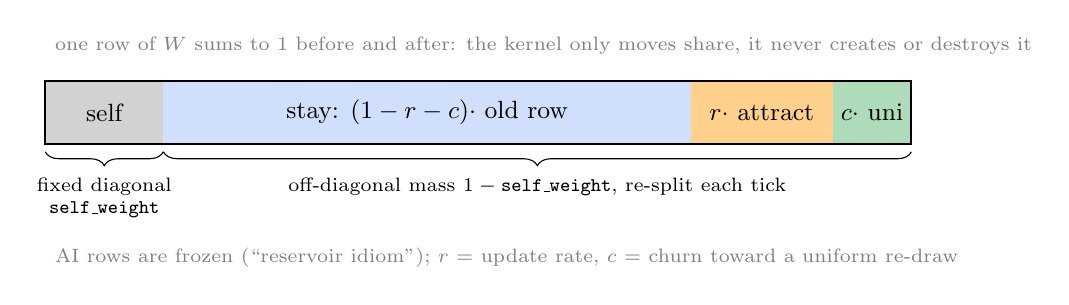
\begin{tikzpicture}[x=1cm,y=1cm, font=\small]
  % one row of W as a bar
  \fill[gray!35] (0,0) rectangle (1.5,0.8);
  \fill[dynamic!25] (1.5,0) rectangle (8.2,0.8);
  \fill[market!45] (8.2,0) rectangle (10.0,0.8);
  \fill[batch0!40] (10.0,0) rectangle (11.0,0.8);
  \draw[thick] (0,0) rectangle (11,0.8);
  \node at (0.75,0.4) {self};
  \node at (4.85,0.4) {stay: $(1-r-c)\cdot$ old row};
  \node at (9.1,0.4) {$r\cdot$ attract};
  \node at (10.5,0.4) {$c\cdot$ uni};
  \draw[decorate, decoration={brace, amplitude=5pt, mirror}] (0,-0.1) -- (1.5,-0.1)
    node[midway, below=6pt, font=\scriptsize, align=center] {fixed diagonal\\ \code{self\_weight}};
  \draw[decorate, decoration={brace, amplitude=5pt, mirror}] (1.5,-0.1) -- (11,-0.1)
    node[midway, below=6pt, font=\scriptsize] {off-diagonal mass $1-\code{self\_weight}$, re-split each tick};
  \node[anchor=west, font=\scriptsize, text=gray] at (0,1.25)
    {one row of $W$ sums to 1 before and after: the kernel only moves share, it never creates or destroys it};
  \node[anchor=west, font=\scriptsize, text=gray] at (0,-1.45)
    {AI rows are frozen (``reservoir idiom''); $r$ = update rate, $c$ = churn toward a uniform re-draw};
\end{tikzpicture}
\end{center}

\noindent Only \code{ledger\_society} calls the shared function. The two older models
keep inlined copies until a refactor proven bit-identical replaces them, and
\code{delegative\_polity}'s copy is a declared fork with exactly three differences.
A point the suite document raises against itself: if attention and delegation are one
object, the culture and politics domains are not independent evidence.

\subsection{\code{coupled\_society}: three domains, one population}

The three substrates' own transforms run on one population: the same humans supply
labor, hold culture and grant attention. One dial $\kappa$ scales five couplings; at
$\kappa=0$ each writes its neutral value, so a $\kappa$ run and a $\kappa=0$ run on the
same key form a causal twin.

\begin{center}
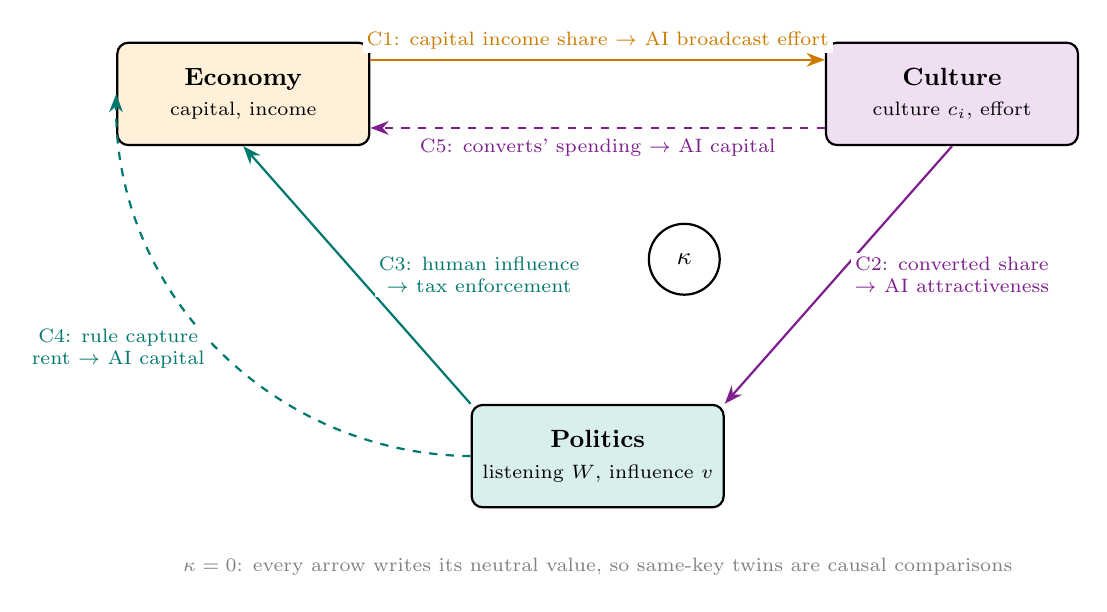
\begin{tikzpicture}[
  dom/.style={draw, thick, rounded corners, minimum width=3.2cm, minimum height=1.3cm, align=center, font=\small},
  ch/.style={-{Stealth}, thick},
  lab/.style={font=\scriptsize, align=center, fill=white, inner sep=1.5pt},
]
\node[dom, fill=market!15]    (eco) at (0,0)    {\textbf{Economy}\\\scriptsize capital, income};
\node[dom, fill=network!15]   (cul) at (9,0)    {\textbf{Culture}\\\scriptsize culture $c_i$, effort};
\node[dom, fill=democracy!15] (pol) at (4.5,-4.6) {\textbf{Politics}\\\scriptsize listening $W$, influence $v$};
\draw[ch, market!80!black] (eco.15) -- node[lab, above=2pt] {C1: capital income share $\to$ AI broadcast effort} (cul.165);
\draw[ch, network!80!black, dashed] (cul.195) -- node[lab, below=2pt] {C5: converts' spending $\to$ AI capital} (eco.345);
\draw[ch, network!80!black] (cul.south) -- node[lab, right=4pt] {C2: converted share\\$\to$ AI attractiveness} (pol.north east);
\draw[ch, democracy!80!black] (pol.north west) -- node[lab, right=6pt] {C3: human influence\\$\to$ tax enforcement} (eco.south);
\draw[ch, democracy!80!black, dashed] (pol.west) to[bend left=45] node[lab, left=3pt] {C4: rule capture\\rent $\to$ AI capital} (eco.west);
\node[draw, circle, thick, minimum size=0.9cm, font=\small] (k) at (5.6,-2.1) {$\kappa$};
\node[font=\scriptsize, text=gray, align=center] at (4.5,-6.0)
  {$\kappa=0$: every arrow writes its neutral value, so same-key twins are causal comparisons};
\end{tikzpicture}
\end{center}

\noindent C4 and C5 were added after review on 27 July because without them the
coupled and sealed economies were bit-identical: the economy drove the others and
nothing drove it back. That provenance matters for any claim about the flywheel, so it
is stated here. Each domain runs on its own clock; between firings the other domains
read stale state, which makes the schedule the composition operator.

The model's headline number is now known to depend on how coupling is implemented
(Section~\ref{sec:flip}). Its own card adds: ``the gains' magnitudes ARE the result's
scale; only the sign/ordering claims are robust.''

\subsection{Where the floors sit}

Every model above has a frozen AI reservoir and one assumption that holds the human
share off zero. The cards now name each one.

\begin{center}
\begin{tabular}{@{}p{3.1cm}p{3.6cm}p{3.6cm}p{4.2cm}@{}}
\toprule
\textbf{Domain} & \textbf{What holds it up} & \textbf{Repo's label} & \textbf{Setup} \\
\midrule
Culture & constant reversion $\rho$ & manufactured: $\approx$0.59 $\to$ 0.008 at $\rho=0$ & coupled model, 6 seeds, $T=500$, one key, no interval \\
Attention & frozen AI rows point at humans & structural: $\approx$0.45--0.50, insensitive to self-weight & same audit \\
Economy & none found & income share 0.07 at $T=500$, 0.018 at $T=1500$ & same audit, all couplings on \\
Delegation & four dialled floors & ``an assumption, not a finding'' & \code{delegative\_polity} card \\
Percepts (WP2) & the anchor $1-\lambda$ & analytic floor $\frac{1-\lambda}{1-\lambda s}$ & offline solve, exact \\
\bottomrule
\end{tabular}
\end{center}

\noindent A four-reader cold read of the lab's assumption cards on 27 July asked for
exactly this: name the floor on every card, in the slider's language.

%% ================================================================
\section{The Economy: Automation With an Owner}

The previous roll-up found that the old economic model assumed its own collapse. The
response was a register of economies. This period added the member written for the
WP1 paper, \code{capital\_economy}, forked from \code{io\_economy}. Its one-line
description: ``A network of recipes in which automation has an owner: AI systems hold
capital that earns the automation slice of sector value added and must pay upkeep out
of revenue before it can compound.''

\textbf{Specification first.} The specification was written, refereed twice and revised
before any code, and it committed a prediction before any sweep: below a survival
threshold
\[
e^* = \frac{\delta/s + m}{v}
\]
(depreciation $\delta$, reinvestment rate $s$, upkeep per unit of capital $m$, sector
value-added coefficient $v$), AI capital cannot pay its upkeep and dies out whatever its
start; above it, capital compounds until it saturates. The referee's own text is not in
the repository, so this document does not attempt a defect-by-defect table.

\subsection{The model}

Twenty households, six sectors (the first makes machines that every other sector uses)
and six AI owners that arrive on a schedule. Recipes are a fixed Leontief matrix $A$.
The economy starts exactly at its people-only steady state.

\begin{algorithm}[H]
\caption{One tick of \code{capital\_economy}}
\begin{algorithmic}[1]
\Require output $x$, wealth $W$, income $y$, owner capital $K_i$, public capital $K^{\text{pub}}_j$, efficiency $e$
\State \textsc{Spend:} household budget $(1-\sigma_s)\max(y_h,0) + \sigma_d W_h$, split by preferences into demand $d_h$
\State \textsc{Arrive:} a scheduled owner activates with seed capital, split $1-\omega$ private and $\omega$ public
\State \textsc{Rebalance:} $x \gets \max(Ax + d_h + d_k,\, 0)$ \Comment{one step toward the Leontief solution}
\State \textsc{Distribute:} automation share $a_j = eK_j/(eK_j+1)$; labor gets $(1-a_j)v_jx_j$, capital $a_jv_jx_j$ pro rata
\State \hspace{1.6em} upkeep paid $=\min(\text{rev}, mK)$; profit $\pi_i = \text{rev}_i - mK_i$; a loss is charged to the stock, not paid
\State \textsc{Mechanism slot:} for example a tax on AI capital income, redistributed to households
\State \textsc{Accumulate:} $K_i \gets (1-\delta)K_i + (1-\omega)\, r s [\pi_i]_+$; unspent profit stays in the owner's hoard
\State \textsc{Grow:} $e \gets \min\big(e_{\max},\, e(1+g+\gamma e)\big)$ once the first owner has arrived
\end{algorithmic}
\end{algorithm}

\noindent The closure parameter $r\in[0,1]$ scales what owners spend. What they do not
spend stays in their hoard: demand stalls, but money is never lost. The parent model's
version leaked money; this fork repairs that on purpose.

\begin{center}
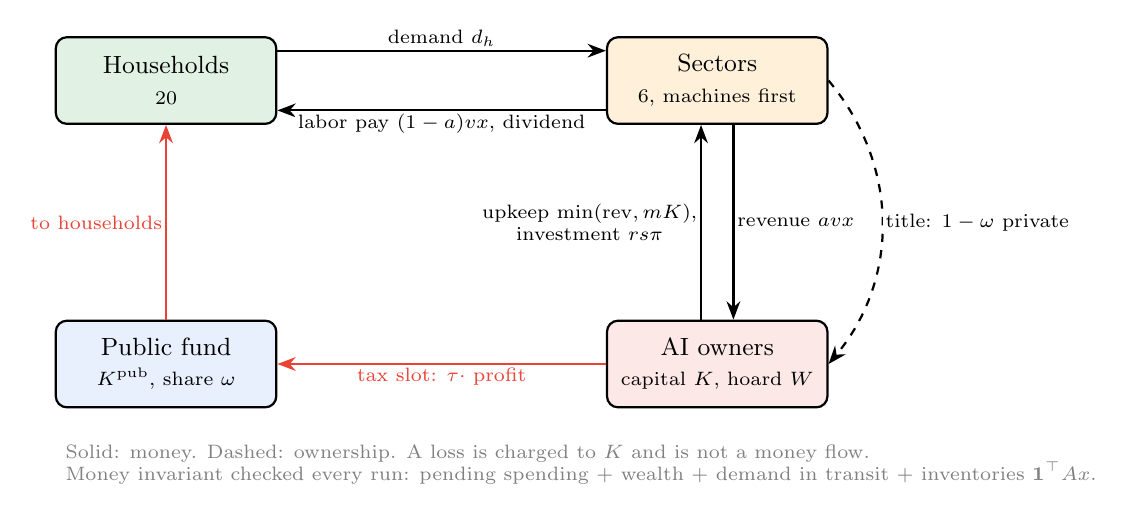
\begin{tikzpicture}[
  box/.style={draw, thick, rounded corners, minimum width=2.8cm, minimum height=1.1cm, align=center, font=\small},
  money/.style={-{Stealth}, thick},
  goods/.style={-{Stealth}, thick, dashed},
  lab/.style={font=\scriptsize, align=center, fill=white, inner sep=1pt},
]
\node[box, fill=batch0!15]  (hh)  at (0,0)    {Households\\\scriptsize 20};
\node[box, fill=market!15]  (sec) at (7,0)    {Sectors\\\scriptsize 6, machines first};
\node[box, fill=static!12]  (ai)  at (7,-3.6) {AI owners\\\scriptsize capital $K$, hoard $W$};
\node[box, fill=dynamic!12] (pub) at (0,-3.6) {Public fund\\\scriptsize $K^{\text{pub}}$, share $\omega$};
\draw[money] (hh.15) -- node[lab, above] {demand $d_h$} (sec.165);
\draw[money] (sec.195) -- node[lab, below] {labor pay $(1-a)vx$, dividend} (hh.345);
\draw[money] (sec.290) -- node[lab, right] {revenue $avx$} (ai.70);
\draw[money] (ai.110) -- node[lab, left] {upkeep $\min(\text{rev},mK)$,\\investment $rs\pi$} (sec.250);
\draw[money, static] (ai.west) -- node[lab, below] {tax slot: $\tau\cdot$ profit} (pub.east);
\draw[money, static] (pub.north) -- node[lab, left] {to households} (hh.south);
\draw[goods] (sec.east) to[bend left=40] node[lab, right] {title: $1-\omega$ private} (ai.east);
\node[font=\scriptsize, text=gray, align=left, anchor=north west] at (-1.4,-4.5)
  {Solid: money. Dashed: ownership. A loss is charged to $K$ and is not a money flow.\\
   Money invariant checked every run: pending spending + wealth + demand in transit + inventories $\mathbf{1}^\top Ax$.};
\end{tikzpicture}
\end{center}

\subsection{The validation ladder}

Eleven rungs, each a test that runs with the suite. They check the mechanism, on one
seed, and are not experiments.

\begin{center}
\begin{tabular}{@{}rp{3.6cm}p{9.6cm}@{}}
\toprule
& \textbf{Rung} & \textbf{What it checks} \\
\midrule
1 & Limit equivalence & no arrivals: output flat at the Leontief point, money drift below $10^{-5}$ \\
2 & The knee & at half the lowest $e^*$ capital dies; at twice the highest it compounds \\
3 & Human share & 1 without AI; at $e=8$ it falls by more than 0.2 \\
4 & Conservation & money conserved at $r \in \{1, 0.5, 0\}$ \\
5 & Conservation with a tax & added after the bug below \\
6 & Fault injection & two planted bug classes must be caught; tests the probe, not the model \\
7 & Eradication band & capital that compounds untaxed dies under a tax of 0.8 \\
8 & Two fund designs & a dividend fund holds the public share at $\omega$; a reinvesting fund approaches 1 \\
9 & Decoupling & AI wealth share stays high while output depends on the closure $r$ \\
10 & Resource manifest & every state field is typed in \code{resources.py} \\
11 & Capability growth & static $e$ never moves; growth lowers the human share; second-order growth is faster \\
\bottomrule
\end{tabular}
\end{center}

\noindent \textbf{A bug the ladder missed.} With a tax in the mechanism slot, the money
check reported a drift near $2\times10^{-2}$ instead of float rounding. The tax writes a
negative bookkeeping record on owner slots that no rule reads, and the money counter
summed it, counting the tax twice. ``The dynamics were never at fault; the instrument
was.'' It survived because the conservation rung ran only with an empty mechanism slot.
It was found when the model was ported to the web playground and the port disagreed
with its source. Rung 5 now covers it.

\textbf{Predictions the implementation contradicted}, each reported rather than
retuned: the money invariant needed an inventory term, since the first version leaked
2.9\% over 200 ticks; the specification's claim that moving ownership to a public fund
leaves the aggregate unchanged was false in both fund designs; and output has an
interior minimum in $r$, because extreme stalling starves the automation itself.

\subsection{The experiments}

Common setup: \code{capital\_economy} at defaults except the swept value, 8 shared seeds
from one key, $T=400$, means over the last quarter, bootstrap 95\% intervals over seeds.
The 8 seeds vary only household preference noise, so the intervals describe that noise
and not parameter uncertainty.

\begin{itemize}
\item \textbf{E1, the knee.} Late private capital is zero at $e \le 0.2$ and positive
  and rising from $e=0.3$, at both $s=0.25$ and $s=0.5$. The grid step is 0.1, so the
  knee is located only to within $[0.2, 0.3]$; the predicted edge for the machine
  sector, about 0.26--0.28, lies in that interval. The upper end of the predicted band
  shows no second transition.
\item \textbf{E2, the closure.} Output falls from 27.0 to 15.6 as $r$ falls from 1 to
  0.25, then rises to 19.7 at $r=0.05$: the minimum is interior. The AI wealth share
  stays near 0.5 for $r \ge 0.25$ and drops to 0.27 at $r=0.05$, because the AI capital
  stock itself is failing.
\item \textbf{E3, defenses.} Raising the tax lowers private capital monotonically and
  raises household income, at a small output cost. At the default $e=0.55$ the tax
  lowers capital but does not eradicate it; eradication is shown only by the
  single-seed ladder rung.
\item \textbf{E5, capability.} The late human share of value added falls as $e$ rises
  across 0.1 to 16: 1.00, then 0.444 at the default, then 0.032 at $e=16$, with
  intervals in the results file. The committed law $\min(1, e^*/e)$ is an upper bound the
  measurement sits below, except at $e=16$ where the prediction is inside the interval.
  The commit calls this ``no interior floor''. Its scope is one parameter set, static
  capability, fixed prices and fixed-rule owners, over that range of $e$.
\item \textbf{E6, growth.} Every growing capability model hits the numerical cap
  $e=64$ within the run, so the late shares cannot rank the growth types. What is
  tested is timing: on the ladder, second-order growth crosses $8e_0$ sooner.
\end{itemize}

\noindent The paper itself moved to the project's notes; the repository holds code
only, and \code{figures.py} regenerates every figure from the results file.

%% ================================================================
\section{The GD Suite and Its Shared Model}

\subsection{The suite, v0.1}

{\sloppy The models were gathered into a named suite with one model per role. It is
defined in \code{environments/suites.py} as \code{GRADUAL\_DISEMPOWERMENT}.\par}

\begin{center}
\begin{tabular}{@{}llll@{}}
\toprule
\textbf{Role} & \textbf{Model} & \textbf{Paper} & \textbf{One line} \\
\midrule
economy  & \code{capital\_economy}    & WP1 & money flows; automation splits value added \\
culture  & \code{influence\_exchange} & WP2 & belief averaging over drifting attention \\
politics & \code{delegative\_polity}  & WP3 & delegated ballots set a tax by weighted median \\
coupled  & \code{coupled\_society}    & none & the old coupling, kept as the baseline \\
\bottomrule
\end{tabular}
\end{center}

\noindent \code{ledger\_society}, below, is the candidate for the coupled slot at v0.2,
gated on a clean comparison against \code{coupled\_society}. It is not in v0.1.

\subsection{Why the coupling was rewritten}

The design review of \code{coupled\_society} found three problems. Three of its five
channels ``mint influence for free'': influence followed an income share with nothing
spent, so the question of where actors route resources was not expressible in the
model. Every channel tested whether an agent was an AI, so ``a human plutocrat cannot
buy reach; the falsifying experiment cannot be run.'' And one unitless dial $\kappa$
gated five different channels.

The rewrite makes cross-domain influence a matter of spending. In the design's words:
``cross-domain influence is never a modulation, it is spending.'' Conversion rates
then have units, and conservation makes bugs announce themselves.

\subsection{\code{ledger\_society}: three conserved ledgers on one population}

Twenty humans and six AI actors hold three ledgers. Money is a stock that is minted by
production and leaves through declared sinks. Attention and ballots are row-stochastic
matrices that the shared kernel reallocates; they are never spent.

\begin{center}
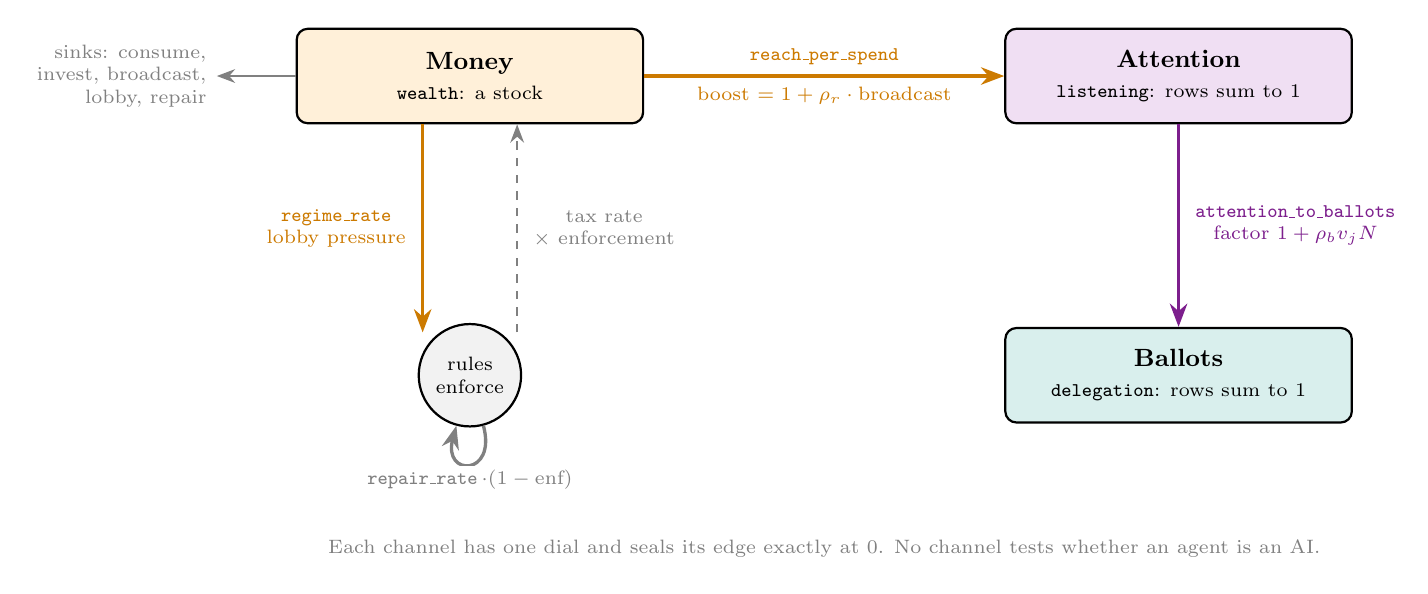
\begin{tikzpicture}[
  led/.style={draw, thick, rounded corners, minimum width=4.4cm, minimum height=1.2cm, align=center, font=\small},
  ch/.style={-{Stealth}, very thick},
  lab/.style={font=\scriptsize, align=center, fill=white, inner sep=1.5pt},
]
\node[led, fill=market!15]    (money) at (0,0)     {\textbf{Money}\\\scriptsize \code{wealth}: a stock};
\node[led, fill=network!15]   (att)   at (9,0)     {\textbf{Attention}\\\scriptsize \code{listening}: rows sum to 1};
\node[led, fill=democracy!15] (bal)   at (9,-3.8)  {\textbf{Ballots}\\\scriptsize \code{delegation}: rows sum to 1};
\node[draw, thick, circle, minimum size=1.3cm, align=center, font=\scriptsize, fill=gray!10] (rules) at (0,-3.8) {rules\\enforce};
\draw[ch, market!80!black] (money) -- node[lab, above=2pt] {\code{reach\_per\_spend}}
  node[lab, below=2pt] {boost $=1+\rho_r\cdot\text{broadcast}$} (att);
\draw[ch, network!80!black] (att) -- node[lab, right=4pt] {\code{attention\_to\_ballots}\\factor $1+\rho_b v_j N$} (bal);
\draw[ch, market!80!black] ($(money.south)+(-0.6,0)$) -- node[lab, left=4pt] {\code{regime\_rate}\\lobby pressure} ($(rules.north)+(-0.6,-0.12)$);
\draw[-{Stealth}, thick, gray, dashed] ($(rules.north)+(0.6,-0.12)$) -- node[lab, right=4pt] {tax rate\\$\times$ enforcement} ($(money.south)+(0.6,0)$);
\draw[ch, gray] (rules) to[loop below, looseness=5] node[lab, below] {\code{repair\_rate}$\,\cdot(1-\text{enf})$} (rules);
\draw[-{Stealth}, thick, gray] (money.west) -- ++(-1.0,0) node[left, font=\scriptsize, align=right] {sinks: consume,\\invest, broadcast,\\lobby, repair};
\node[font=\scriptsize, text=gray, align=center] at (4.5,-6.0)
  {Each channel has one dial and seals its edge exactly at 0. No channel tests whether an agent is an AI.};
\end{tikzpicture}
\end{center}

\begin{algorithm}[H]
\caption{One tick of \code{ledger\_society} (program order derived from declared reads and writes)}
\begin{algorithmic}[1]
\Require capital $k$, income $y$, wealth $w$, listening $W$, delegation $D$, enforcement, efficiency $e$
\State \textsc{Arrive, produce:} AI actors gain seed capital on schedule; $a = eK/(eK+H)$, output $Y=H(1+a)$; humans get labor $(1-a)Y/H$, everyone capital $aYk_i/K$
\State \textsc{Tax:} rate $=$ last tick's \code{policy\_target} $\times$ enforcement; the take is paid out equally to humans
\State \textsc{Allocate:} budget $y_i + 0.15\,w_i$ split over consume, invest, broadcast, lobby, save
\State \textsc{Build capital, grow:} $k \gets 0.95k + \text{invest}$; $e$ grows to a ceiling
\State \textsc{Reach:} attractiveness boost $1 + \rho_r \cdot \text{cut} \cdot \text{broadcast}_i$ \Comment{money $\to$ attention}
\State \textsc{Rewire listening:} shared kernel toward $(v_j+\epsilon)^{\gamma_w}\cdot\text{boost}_j$; AI rows frozen
\State \textsc{Attention influence, belief:} $v \gets W^\top v$, normalised; human beliefs averaged with an anchor
\State \textsc{Rewire delegation:} shared kernel toward $(u_j+\epsilon)\cdot(1+\rho_b v_j N)$, with churn \Comment{attention $\to$ ballots}
\State \textsc{Tally, declare, vote:} power $u$; weighted median of positions sets \code{policy\_target}
\State \textsc{Regime:} enf $\gets \mathrm{clip}\big(\text{enf} + \rho_g\cdot\text{pressure} + \text{repair}\cdot(1-\text{enf}) - \text{entrench}\cdot\text{over}\big)$ \Comment{money $\to$ rules}
\State \textsc{Mechanisms, step counter}
\end{algorithmic}
\end{algorithm}

\noindent Lobby pressure has an endogenous direction: an agent's stance is the sign of
its net redistribution transfer, so the winners of the current rules defend them.
\textbf{Self-repair} was added on 30 July because without a restoring force any
sustained pressure was a ratchet: a probe found \code{regime\_rate} 0.005 alone
collapsing enforcement by $t=400$. That probe's seeds are not recorded, so it is
stated here only as an ordering.

\textbf{The live policy plan.} With \code{policy\_horizon} $>0$ the state carries a
$(T,4)$ array of defense levels per tick: a levy on AI wealth, a repair drip, a reach
cut and a sortition rate. The plan is data, not configuration, so every plan of the
same length shares one compiled program. Every lever is exactly neutral at zero.

\subsection{A floor that read as a finding}

The AI rows of both kernels are frozen at their random starting draw, which points
them mostly at humans: about 0.69 of an AI row's attention and 0.58 of its ballots, for
the whole run. On 1 August this was found to hold the human attention share above
about 0.45 under every dial setting tried; the runs ``all landed on 0.4505'' (8 seeds,
no interval; the claim is that the floor exists, not its size). In the design
document's words: ``That is a property of the initial draw, not of the coupling, and it
had been reading as a result.'' A dial, \code{ai\_insularity}, now redirects frozen AI
rows toward other AI actors; at 0 it is bit-identical to the old model. It is a
workaround, not a resolution: letting AI rows drift would make who the AI attends to
endogenous, and that is an open decision.

\subsection{The coupling result depends on the implementation}\label{sec:flip}

The \emph{transfer gap} is the composite human share in a sealed model minus the
composite in the coupled model. Under the old coupling, the gap was reported larger
with defenses than without (0.128 against 0.109; 8 seeds, one key, no interval). The
card read this as defenses losing more of their protection to coupling than having
none would.

Under the ledger coupling, on 1 August, with 64 paired seeds, $T=400$ and a late
window, the gap was $0.2420 \pm 0.0045$ undefended and $0.0876 \pm 0.0033$ defended:
a paired difference of $-0.1545 \pm 0.0032$ (95\% $t$-interval), with no seed on the
other side. The sign flips. But the defenses were not the same instruments in the two
models: attached mechanisms in one, in-transform dials in the other. ``Two things
changed at once, so the reversal is not yet attributable to the coupling implementation
rather than to the defense instruments.'' What this licenses is narrower: the finding
is implementation-sensitive, and the earlier transfer-gap numbers stay out of any
claim. A comparison with one defense pair present in both models is the next step.

\subsection{Dial lattices: the web shows, the engine computes}

\code{experiments/gd\_bundles} sweeps each suite model over a grid of three dials
offline and writes a versioned static bundle: a manifest, per-cell scalars with
bootstrap intervals, and one representative trajectory per cell. The web playground
selects among precomputed real runs and computes nothing. Two of the grids are imported
from the WP experiment configurations, so the papers' sweeps and the playground's dials
cannot drift apart. Each bundle carries committed ordering expectations, and a miss
exits with an error; whether the current bundles pass is not recorded in the
repository, so this document does not say.

\subsection{The game: two routes, both recorded dead}

On 31 July two games were built on \code{ledger\_society}. Route A precomputed a tree
of choices: three intervention windows, five defense cards, 73 paths across three towns,
walked in the browser. Route B put continuous levers behind a service that re-ran the
model per request. On 1 August both were judged not worth continuing. From the
postmortem: route A is ``a game with about three choices in a whole run. That is the
ceiling of the route, not a bug in this instance of it''; route B is ``a form full of
parameters a new player does not understand''. The diagnosis: ``We derived a game from
the engine we had, instead of designing a game and then asking what engine it needs.''
A batch simulator that scans a fixed number of steps allows exactly those two shapes;
``configurability is not interactivity''.

The postmortem names its own weak points: the verdict was one person's, after one day,
without players, and the claim that the two routes exhaust what a batch engine allows
is ``an argument, not a proof''. The code that exists because of the game (lever
families, the policy plan, whole-run metrics) stays, marked, and its presence is not a
reason to revive either route.

Two engine findings survive the game. The \code{belief} field in \code{ledger\_society}
feeds no scored outcome: changing susceptibility from 0.7 to 0.4 moved no ledger metric
to four decimals. And sealing conventions must be tested inside the compiled scan, not
only eagerly: a neutral plan was bit-identical eagerly but about one unit in the last
place off under \code{lax.scan}.

%% ================================================================
\section{The Engine: Measure, Then Change}

Nothing in this section changes a model or a reported number, unless a subsection says
otherwise. One concern runs through it. Float32 arithmetic can give different last
digits for the same formula when the computation is batched or compiled differently,
and in models with thresholds such a difference can grow: in \code{ledger\_society} a
rounding difference once crossed an enforcement threshold and rewired the delegation
matrix within 12 steps. So each change below either keeps results bit-identical or says
in writing where and by how much it does not.

\subsection{Reducers: metrics folded into the loop}

A metric used to score the stacked trajectory: the simulation wrote every state's
readout for every step, and a function then walked that block once to return, usually,
one number. A \emph{Reducer} does the same fold inside the loop, keeping only an
accumulator.

\begin{center}
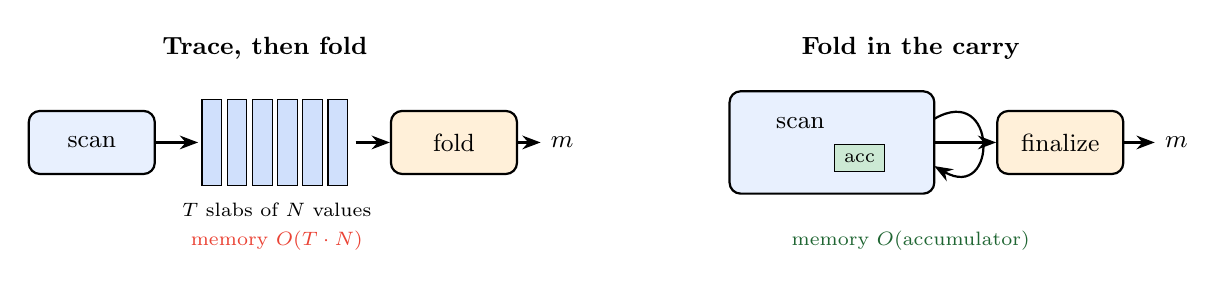
\begin{tikzpicture}[
  blk/.style={draw, thick, rounded corners, minimum width=1.6cm, minimum height=0.8cm, font=\small},
  arr/.style={-{Stealth}, thick},
]
% left: trace then fold
\node[font=\small\bfseries] at (2.2,1.2) {Trace, then fold};
\node[blk, fill=dynamic!12] (s1) at (0,0) {scan};
\foreach \i in {0,...,5} {
  \draw[fill=dynamic!25] (1.4+0.32*\i, -0.55) rectangle ++(0.25, 1.1);
}
\node[font=\scriptsize] at (2.35,-0.85) {$T$ slabs of $N$ values};
\node[blk, fill=market!15] (f1) at (4.6,0) {fold};
\draw[arr] (s1) -- (1.35,0);
\draw[arr] (3.35,0) -- (f1);
\draw[arr] (f1) -- ++(1.1,0) node[right, font=\small] {$m$};
\node[font=\scriptsize, text=static] at (2.35,-1.25) {memory $O(T\cdot N)$};
% right: carry
\node[font=\small\bfseries] at (10.4,1.2) {Fold in the carry};
\node[blk, fill=dynamic!12, minimum width=2.6cm, minimum height=1.3cm] (s2) at (9.4,0) {};
\node[font=\small] at (9.0,0.25) {scan};
\node[draw, fill=batch0!25, font=\scriptsize] at (9.75,-0.2) {acc};
\draw[arr] (10.7,0.3) to[out=30, in=-30, looseness=4] (10.7,-0.3);
\node[blk, fill=market!15] (fz) at (12.3,0) {finalize};
\draw[arr] (s2) -- (fz);
\draw[arr] (fz) -- ++(1.2,0) node[right, font=\small] {$m$};
\node[font=\scriptsize, text=batch0!60!black] at (10.4,-1.25) {memory $O(\text{accumulator})$};
\end{tikzpicture}
\end{center}

\begin{algorithm}[H]
\caption{\code{run\_scan\_reduce}: a scan with reducers in the carry}
\begin{algorithmic}[1]
\Require reducers $\{(\text{init}, \text{update}, \text{finalize})\}$, sorted by name for a fixed carry order
\State $\text{acc} \gets \text{init}(s_0, T)$ for each reducer \Comment{an identity element: 0 for a sum, $-\infty$ for a max}
\For{$t = 0, \dots, T-1$} \Comment{one \code{lax.scan}}
  \State $s \gets \text{round}(s, t, k_t)$
  \State $\text{acc} \gets \text{update}(\text{acc}, s, t, T)$ \Comment{branch-free in $t$}
\EndFor
\State \Return $\text{finalize}(\text{acc}, T)$ for each reducer
\end{algorithmic}
\end{algorithm}

\noindent The start value must be an identity element, never the readout of the
initial state: otherwise the fold covers $T+1$ states and quietly includes one the
trace never sees. A survey of every metric in the library found four shapes and no
metric that needs the full time-by-agent block. Results match the trace-based metrics
to float32 rounding, not bit for bit, because a streaming sum adds in a different
order. Size, by arithmetic rather than measurement: for \code{value\_contagion} at
$N=5000$, 16 seeds and $T=2000$, the state is 0.45\,MB and the stacked trace 1.28\,GB.

\subsection{Sparse networks, typed homophily, a spectral readout}

Adjacency can now be stored sparse, so cost tracks edges rather than node pairs. Every
generator still builds the dense matrix, so the edge distribution is the same; the
number of stored entries is a fixed bound set from the configuration, because every
seed in a batch must share array shapes. If a concrete graph would overflow the bound,
conversion raises, since silent truncation would look like a valid sparser graph.
\code{typed\_homophily} keeps expected degree fixed as separation rises, and
\code{fiedler\_partition\_alignment} reads separation back from the network as the
absolute correlation between the sign split of the Laplacian's second eigenvector and
the human/AI labels.

\subsection{\code{system\_graph} and one web exporter}

Every transform declares the fields it reads and writes, which the pipeline compiler
already uses to order steps. \code{system\_graph} emits the same declarations as a
graph: field nodes, transform nodes, and edges from reads and to writes. It reads only
the state's schema, never values, so ``a topology nobody hand-drew and nobody has to
keep in sync''. \code{webexport.trajectory\_payload} became the single producer of the
web trajectory format, and a parity test pins it to the old output byte for byte.

\subsection{\code{perf\_baseline}: where the time goes}

Before touching the engine, it was measured. Provenance for this table: 2026-09-10,
commit \code{09b486f}, jax 0.9.0, CPU with 12 cores, $T=200$, best of 3, every model at
its default size. Engineering measurements, one machine, no interval.

\begin{center}
\begin{tabular}{@{}p{4.6cm}p{9.6cm}@{}}
\toprule
\textbf{Finding} & \textbf{Measured} \\
\midrule
Compile dominates & compiling the scan 0.3--0.9\,s; running 200 steps 1--6\,ms \\
The eager path recompiled & a second eager call cost as much as the first \\
Seeds are nearly free & 32 seeds under \code{vmap} cost 2--8 times one seed \\
Dense adjacency is the ceiling & 7 to 11 times the time for twice the nodes at the top of the range, e.g. \code{ledger\_society} 326\,ms at $N=646$, 2653\,ms at $N=1286$ \\
\bottomrule
\end{tabular}
\end{center}

\noindent The baseline also corrected itself in writing: the quadratic term in
\code{capital\_economy} was later identified (a recipe matrix stored padded to $N\times
N$), and a 1\,h\,42\,min test-suite run did not reproduce (6\,min\,21\,s the same day;
the suite is compile-bound).

\subsection{Compile once per spec}

Every \code{run*} method of \code{EnvSpec} now compiles its scan once per spec and
call signature and keeps the program on the spec. A plain \code{jax.jit} around
\code{run} changed float32 results in 10 of 13 models, for three separate reasons,
each handled.

\begin{enumerate}
\item \textbf{A compiled initial state rounds differently} (9 of 13): XLA fuses its
  arithmetic. Initialisation stays eager, outside the program.
\item \textbf{Fields \code{vmap} leaves unbatched.} The old batch path scanned
  seed-constant fields, such as a fixed network, unbatched. Batching them compiles a
  different program, so each field's batching is recorded and passed on.
\item \textbf{Closed-over arrays become constants} that XLA folds with the host's math
  library. They now reach the program as runtime arguments, as they did eagerly. The
  red-team pass found this one, with a model where a plain jit differs in 1391
  elements.
\end{enumerate}

\begin{algorithm}[H]
\caption{\code{EnvSpec.\_compiled}: one program per call signature}
\begin{algorithmic}[1]
\State $\text{sig} \gets (\text{tag}, \text{id(round\_fn)}, \text{id(trace\_fn)}, \text{static}, \text{tree structure}, \text{shapes and dtypes})$ \Comment{never values}
\If{sig not cached}
  \State $\text{jaxpr}, \text{consts} \gets \code{make\_jaxpr}(f)(\text{inputs})$ \Comment{lifts closed-over arrays into consts}
  \State cache $\code{jit}(\code{eval\_jaxpr}(\text{jaxpr}))$ with consts \emph{as arguments}
\EndIf
\State \Return cached program applied to (consts, inputs)
\end{algorithmic}
\end{algorithm}

\noindent Every model's results stayed bit-identical, held by an exact-equality test
over every registered model. A repeat call fell from 0.19--0.86\,s to 3--15\,ms for one
run, and from 0.25--1.35\,s to 14--73\,ms for 8 seeds (same machine, $T=200$). An
earlier attempt on 11 September had batched every field instead, which moved past
batch results in five models; it was not merged as is. Whether one seed of a batch
should equal a single run is an open decision; today they differ in 6 of 11 default
models, by up to 0.03 in \code{ledger\_society} at $T=50$.

\subsection{Run records: metric identity and the run store}

Every metric now declares a kind (share, concentration, rate, level or index) and a
version, plus an advisory hash of its definition. The hash walks the metric's source
and every helper it reaches, because the first version hashed only the metric's own
text, and a red-team pass showed that halving a helper doubled two metrics with the
hash unchanged.

A run writes a record directory through \code{cilib.runs}.

\begin{center}
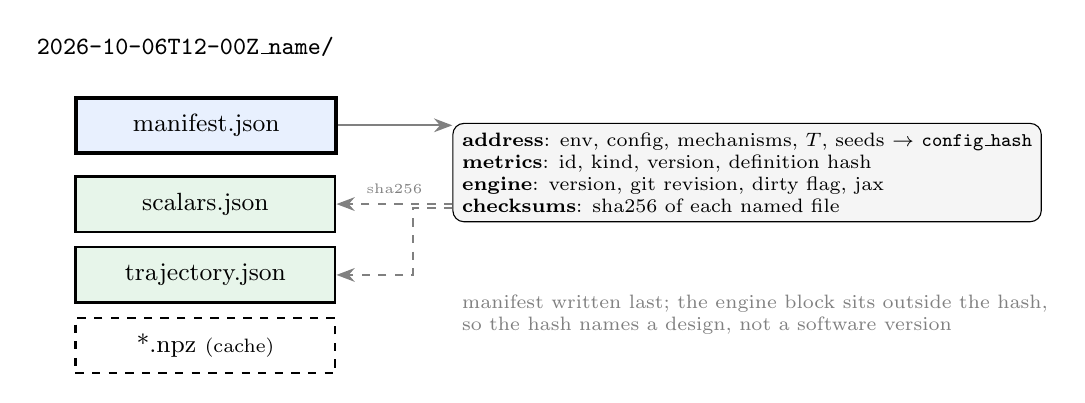
\begin{tikzpicture}[
  file/.style={draw, thick, minimum width=3.3cm, minimum height=0.7cm, font=\small, anchor=west},
  arr/.style={-{Stealth}, thick, gray},
]
\node[font=\small\ttfamily, anchor=west] (dir) at (0,0) {2026-10-06T12-00Z\_name/};
\node[file, fill=dynamic!12, line width=1.4pt] (man) at (0.6,-1.0) {manifest.json};
\node[file, fill=batch0!12] (sc) at (0.6,-2.0) {scalars.json};
\node[file, fill=batch0!12] (tr) at (0.6,-2.9) {trajectory.json};
\node[file, dashed] (npz) at (0.6,-3.8) {*.npz \scriptsize(cache)};
\node[draw, rounded corners, fill=gray!8, align=left, font=\scriptsize, anchor=west] (blk) at (5.4,-1.6)
  {\textbf{address}: env, config, mechanisms, $T$, seeds $\to$ \code{config\_hash}\\
   \textbf{metrics}: id, kind, version, definition hash\\
   \textbf{engine}: version, git revision, dirty flag, jax\\
   \textbf{checksums}: sha256 of each named file};
\draw[arr] (man.east) -- (blk.west |- man.east);
\draw[arr, dashed] (blk.west |- sc.east) -- node[above, font=\tiny] {sha256} (sc.east);
\draw[arr, dashed] ($(blk.west)+(0,-0.45)$) -- ++(-0.5,0) |- (tr.east);
\node[font=\scriptsize, text=gray, anchor=west, align=left] at (5.4,-3.4)
  {manifest written last; the engine block sits outside the hash,\\
   so the hash names a design, not a software version};
\end{tikzpicture}
\end{center}

\noindent Reading a record recomputes the address hash and every checksum, so a
hand-edited run length or a changed file is caught. A missing \code{.npz} is allowed:
it is a cache that can be regenerated. ``One record is one design over its seeds'': the
experiment, not the seed, is the unit.

\subsection{\code{run\_grid}: a grid of settings as one compiled program}

\textbf{The problem.} Seeds were batched, but every other dial was configuration closed
over by the model's functions. Each grid cell needed its own spec and paid its own
compile. A dial stored as an array in the state's global attributes instead reaches the
program as an input, so new values need no new compile.

\begin{algorithm}[H]
\caption{\code{EnvSpec.run\_grid}$(key, S, T, \text{grid}, \text{reducers}, \text{batch}=1)$}
\begin{algorithmic}[1]
\Require grid $=\{\text{global key}: \text{array}(G, \dots)\}$; each key must already be an array in the initial state
\State build the $S$ initial states once, eagerly, and record each field's batching
\Function{cell}{$g$}
  \For{each seed, under \code{vmap}}
    \State $s \gets$ initial state with $\text{global}[k] \gets g[k]$ \Comment{\code{with\_globals}, pure}
    \State run the \code{run\_reduced\_batch} scan from $s$, reducers built from $s$
  \EndFor
\EndFunction
\State \Return \code{lax.map}(\Call{cell}{}, grid, batch size) \Comment{one program for all $G$ cells}
\end{algorithmic}
\end{algorithm}

\noindent Every cell uses the same key, so seed $s$ draws the same random numbers in
every cell, and cells are compared as paired differences over seeds; a new helper,
\code{paired\_diff\_ci}, does that comparison. Cells run one at a time by default. A
first version vectorised the cells and left 7 of 25 cells off the reference numbers by
float32 rounding; one at a time, each cell is exactly the \code{run\_reduced\_batch}
program for its value.

Measured on \code{ledger\_society} at its defaults: 25 cells over \code{churn} and
\code{repair\_rate}, 8 seeds, $T=400$, late-window human shares. One machine, jax 0.9.0,
CPU, 2026-10-06, one run per row, no interval; the equality column is exact.

\begin{center}
\begin{tabular}{@{}lccc@{}}
\toprule
\textbf{Path} & \textbf{First call} & \textbf{Repeat} & \textbf{Cells equal to the loop} \\
\midrule
loop of 25 specs, one compile each & 44.7\,s & & reference \\
\code{run\_grid}, one cell at a time & 3.5\,s & 1.5\,s & 25 of 25, bit for bit \\
\code{run\_grid}, all cells vectorised & 2.3\,s & 0.6\,s & 18 of 25 \\
\bottomrule
\end{tabular}
\end{center}

\noindent Three red-team attackers found two grid keys that had to be refused (the
random key, which the round overwrites, and the step counter, which shifts the clock),
a silent truncation of fractional values given to an integer dial, three test gaps
where the suite passed on deliberately broken code, and one exception to bit-identity:
a reducer start value that the scan never overwrites is computed inside the program and
can be one unit in the last place off. Each is fixed or recorded with its answer in
\code{docs/run-grid-design.md}.

\textbf{Lifting a dial can move numbers.} Making \code{ledger\_society} grid-ready meant
moving its three channel dials into the state. Checked against a snapshot of the old
code at $T=400$, five configurations, every field of every run path: single runs did
not change, but on the seed-batched paths lifting \code{reach\_per\_spend} or
\code{regime\_rate} did. At the defaults the change was about $10^{-7}$; at maximum
coupling it grew to 0.003 in the per-tick human power share. XLA compiles a constant
and a runtime input differently once seeds are under \code{vmap}. Because past results
must not move, the lift sits behind a flag, \code{traced\_channels}, off by default;
with it off, all 798 compared arrays are unchanged. A result made with the flag on says
so and is compared only with results made the same way.

%% ================================================================
\section{Process}

\begin{itemize}
\item \textbf{\code{ROADMAP.md}} is the single source of truth for what the library does
  next. Other status lines derive from it, and a change that lands in the engine ends by
  moving its card.
\item \textbf{\code{STANDARDS.md}, v0.} ``Vary what you are uncertain about; trust what
  survives.'' Claims are orderings between counterfactuals, made with paired seeds and
  an interval, with predictions on record before the sweep and parameters typed as
  anchored, tuned or arbitrary-but-swept.
\item \textbf{Claim discipline.} A number travels with its context or it does not
  travel. Model choices carry their provenance where they are used. Unknowns are written
  down in place. Substantive designs and results get an adversarial pass before they
  are committed, and the attacks are recorded with their answers.
\item \textbf{Paper style.} The reader is a smart high-school student: abstracts in
  words only, no parenthetical asides, no invented vocabulary, and every figure
  regenerated from committed artifacts.
\item \textbf{Code only.} Papers, specifications and planning live outside the
  repository. Router \code{CLAUDE.md} files per area replaced one long file, and
  simulated reader panels were removed from the repository under the rule that they are
  not evidence.
\end{itemize}

%% ================================================================
\section{Open Items}

\begin{itemize}
\item Whether the transfer-gap sign flip comes from the coupling or from the change of
  defense instruments. Needs one defense pair present in both models.
\item AI listening rows: frozen, insular, or drifting under the same kernel.
\item The \code{belief} field in \code{ledger\_society} feeds no scored outcome; it
  either gets a path into the ledgers or culture there means only the shape of the
  attention kernel.
\item The two older models still carry inlined copies of the attachment kernel.
\item Whether one seed of a batch should equal a single run.
\item Sparse or structured adjacency for the ledger models: dense matrices are the
  scaling ceiling, and no sparse-versus-dense timing is committed yet.
\item The WP2 and WP3 experiment results are not in the repository; their designs are.
\item Whether the dial-lattice bundles pass their committed expectations is not
  recorded.
\end{itemize}

\end{document}
